\documentclass[11pt]{amsart}
\usepackage{geometry}                % See geometry.pdf to learn the layout options. There are lots.
\geometry{letterpaper}                   % ... or a4paper or a5paper or ... 
%\geometry{landscape}                % Activate for for rotated page geometry
%\usepackage[parfill]{parskip}    % Activate to begin paragraphs with an empty line rather than an indent
\usepackage{graphicx}
\usepackage{amssymb}
\usepackage{epstopdf}
\usepackage[usenames,dvipsnames]{color}
\usepackage{fancyvrb}
\usepackage{listings}
\usepackage{booktabs,footmisc}
\usepackage{hyperref}
\usepackage[all]{hypcap}

\usepackage{topcapt}
\usepackage{enumerate}
\usepackage[section] {placeins}

 
% include the lines below to use a nicer fixed-width font than the default one
 
\lstset{fancyvrb=true}
\lstset{
	basicstyle=\small\tt,
	identifierstyle=,
	commentstyle=\color{Bittersweet},
	stringstyle=\color{red},
	showstringspaces=false,
	tabsize=3,
	numbers=left,
	captionpos=b,
	xleftmargin=2em
%	numberstyle=\tiny
	%stepnumber=4
	}
\DeclareGraphicsRule{.tif}{png}{.png}{`convert #1 `dirname #1`/`basename #1 .tif`.png}

\title{Repast Simphony System Dynamics Getting Started}
\author{Mark Bragen}
%\date{\today}                                           % Activate to display a given date or no date

\begin{document} 
\maketitle

\section{System Dynamics in Repast Simphony}
New to this release of Repast Simphony is support for developing System Dynamics models from scratch. This release also supports importing existing System Dynamics models into your projects and converting it to a format that can be displayed and manipulated by the System Dynamics Graphical User Interface (GUI). Given the set of equations of the System Dynamics model, Java source code is generated that implements the model. The standard generated code implements the Euler method directly. An alternate form generated for System Dynamics models that meet certain criteria (specified in a later section), is compatible with the Apache ODE Solver library.
This tutorial presents the steps required to create a System Dynamics model in Repast Simphony.
Figure 1 shows the layout of the System Dynamics GUI screen in the Eclipse IDE. The layout is similar to all other Repast Simphony models that are specified via Eclipse. The left-side panel contains all the Repast Simphony projects that have been defined. Displayed in area are all files related to the projects such as source code, generated code, output files, etc. The top-center panel is a tabbed panel in which source code and diagrams can be viewed and edited. Finally, the lower-right panel is a tabbed panel in which console output, search output, System Dynamics model variable properties, etc. will be displayed. The Eclipse IDE is highly configurable and the more experienced users will know that location of these areas can easily be moved into other configurations to suit the needs of the user.\\





\begin{figure}[ht]
\begin{center}
\vspace{.2in}
\centerline {
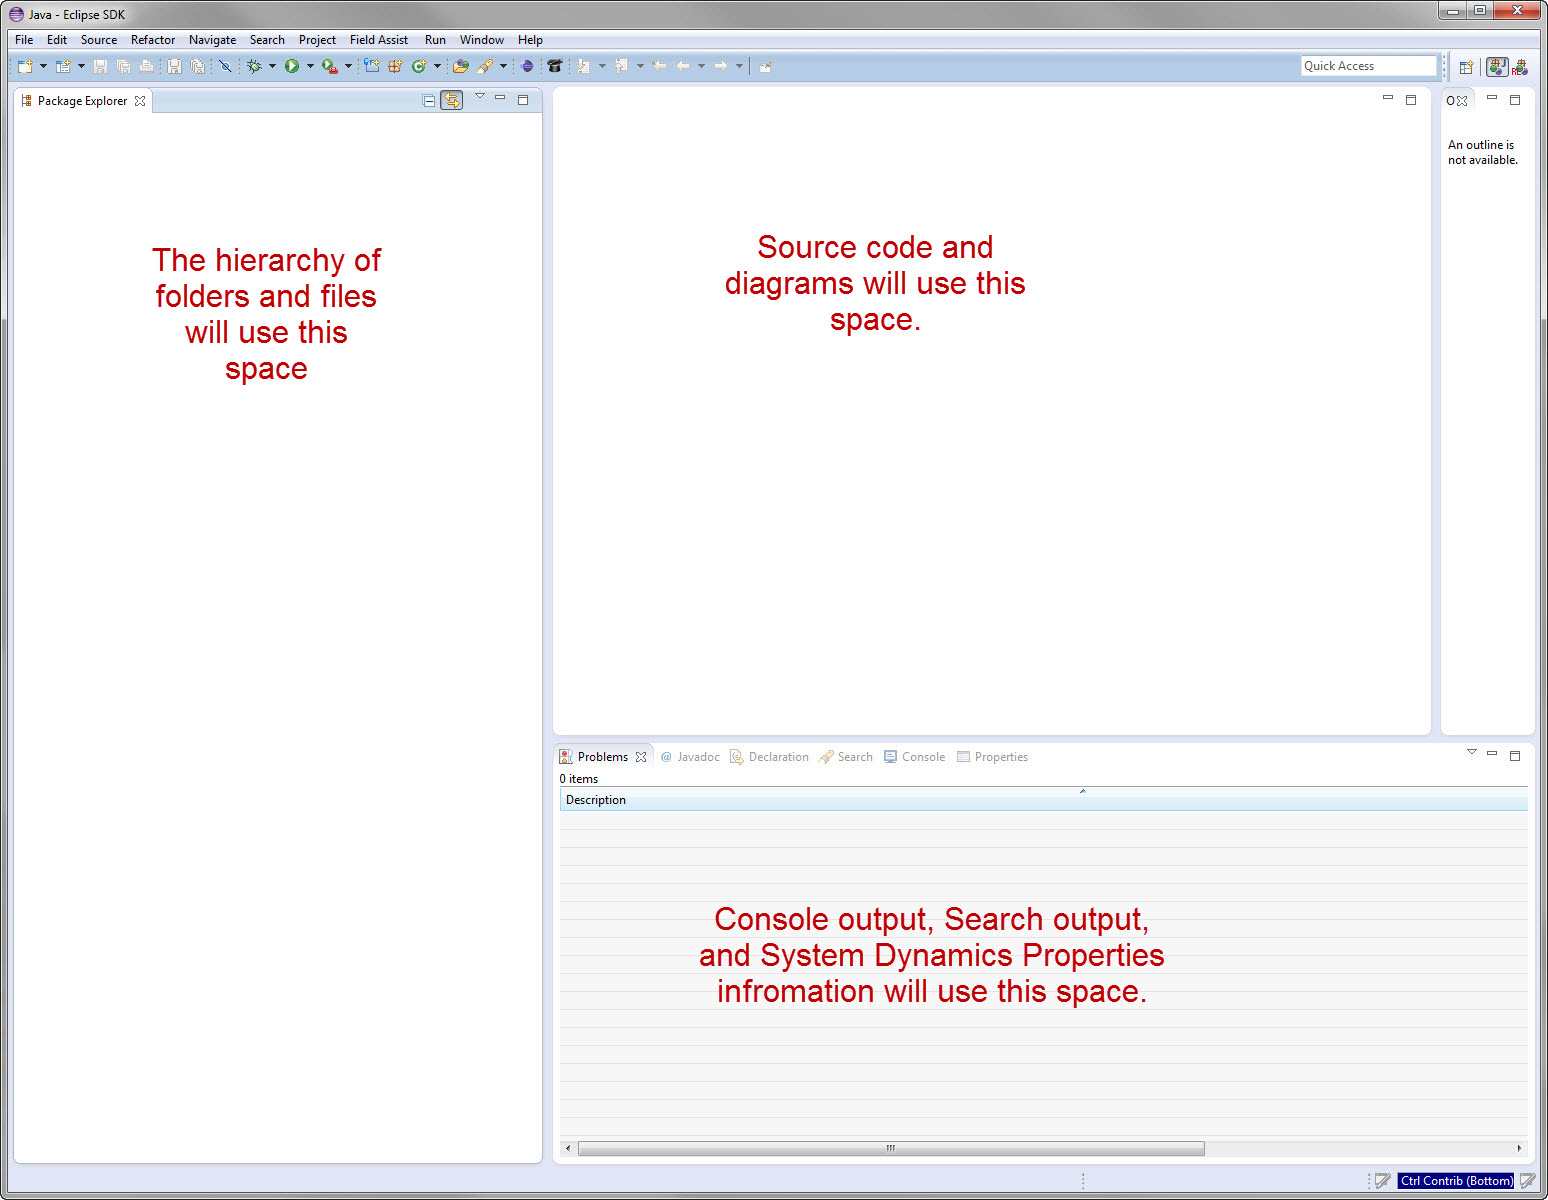
\includegraphics[totalheight=0.5\textheight]{images/001.jpg}
}
\caption{}
\label{fig:001}
\end{center}
\end{figure}

\section{Create a new Repast Simphony Project}
The first step in creating a System Dynamics (SD) model is to create a Repast Simphony project in which the SD model will be located. Figure 2 illustrates how this is done. Right click the mouse in the Project panel to bring up the menus. Navigate from New to Other and left click on Other. Another window will open that lists the available wizards for performing tasks. This is shown in figure 3. Select Repast Simphony Project and left click on the Next button. Another window appears in which you specify the name of the project. See Figure 4. Note that the project name must be unique within your workspace. Left click on Finish to cause the new project wizard to create the required Repast Simphony project structure.



\begin{figure}[ht]
\begin{center}
\vspace{.2in}
\centerline {
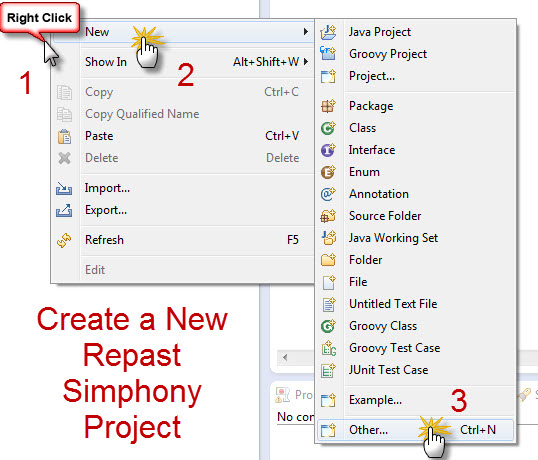
\includegraphics[totalheight=0.35\textheight]{images/002.jpg}
}
\caption{}
\label{fig:002}
\end{center}
\end{figure}




\begin{figure}[ht]
\begin{center}
\vspace{.2in}
\centerline {
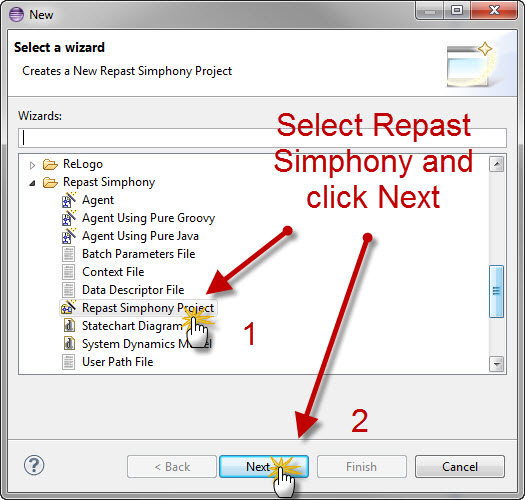
\includegraphics[totalheight=0.35\textheight]{images/003.jpg}
}
\caption{}
\label{fig:003}
\end{center}
\end{figure}




\begin{figure}[ht]
\begin{center}
\vspace{.2in}
\centerline {
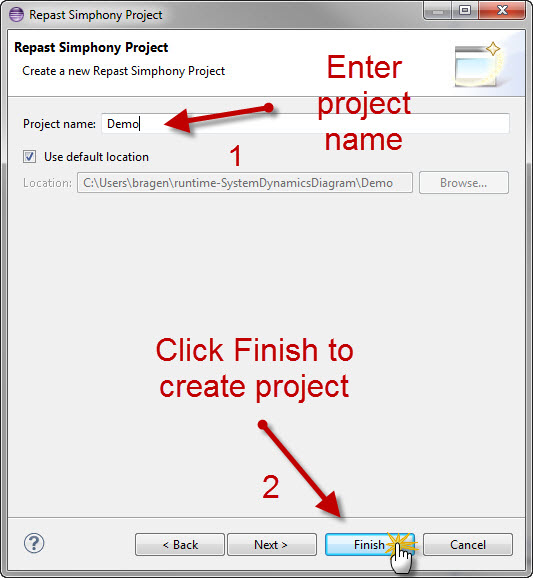
\includegraphics[totalheight=0.35\textheight]{images/004.jpg}
}
\caption{}
\label{fig:004}
\end{center}
\end{figure}

When the create Repast Simphony wizard completes, you will see the scenario directory structure as contained in Figure 5. The wizard automatically created two files under source: ModelInitializer.groovy and ModelInitializer.agent. These files are used by other Repast Simphony modeling techniques and are not required for System Dynamics models. You can delete them from your. Leaving them in the project will not affect your model.


\begin{figure}[ht]
\begin{center}
\vspace{.2in}
\centerline {
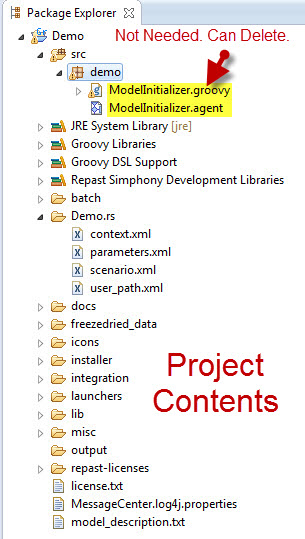
\includegraphics[totalheight=0.35\textheight]{images/005.jpg}
}
\caption{}
\label{fig:005}
\end{center}
\end{figure}

\section{Create an Empty System Dynamics Model}
Now that we have the project created, we need to create an empty System Dynamics model to initialize the dataset in which the model will be stored. Once again, there’s a wizard for that. Right click on the package name demo under the src folder. Navigate to New and Other. Click on Other (See Figure 6). The list of available wizards will appear as it did when the project was being created. Select System Dynamics Model and click on Next (See Figure 7).



\begin{figure}[ht]
\begin{center}
\vspace{.2in}
\centerline {
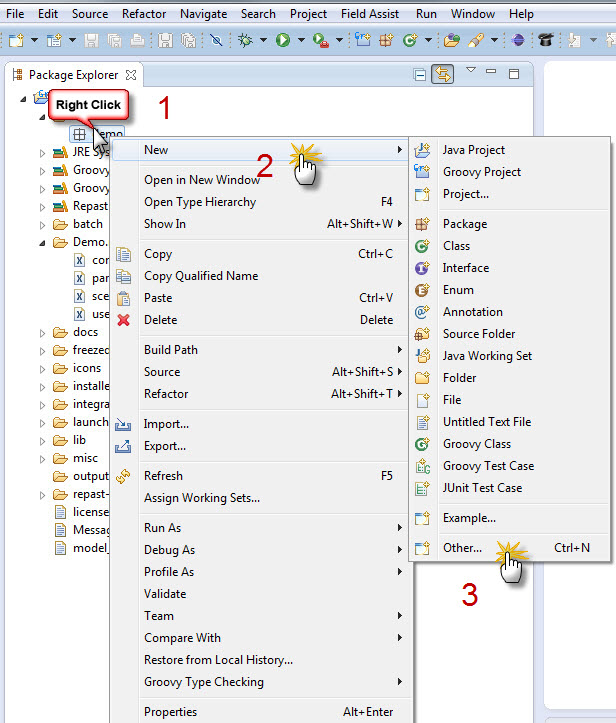
\includegraphics[totalheight=0.4\textheight]{images/006.jpg}
}
\caption{}
\label{fig:006}
\end{center}
\end{figure}




\begin{figure}[ht]
\begin{center}
\vspace{.2in}
\centerline {
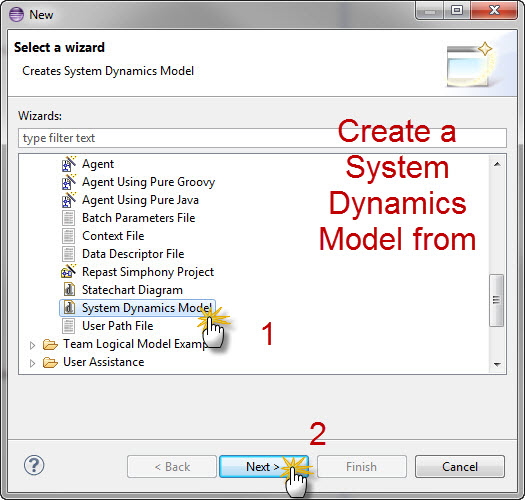
\includegraphics[totalheight=0.35\textheight]{images/007.jpg}
}
\caption{}
\label{fig:007}
\end{center}
\end{figure}

A new window will appear requiring four pieces of information (See Figure 8):

\begin{enumerate}
\item The folder into which to place the model file. This is initialized to the folder that was selected when the New menu was selected.
\item The name of the model file (.rsd extension). This is initialized to default.rsd.
\item The class name. This is the name of the Java class that will be generated. It is initially blank and must be supplied.
\item The package name. This is the Java package name into which the class will be placed. It is initially blank and must be supplied.
\end{enumerate}
\vspace{.2in}

Click on Finish to complete the process of creating a new SD model.



\begin{figure}[ht]
\begin{center}
\vspace{.2in}
\centerline {
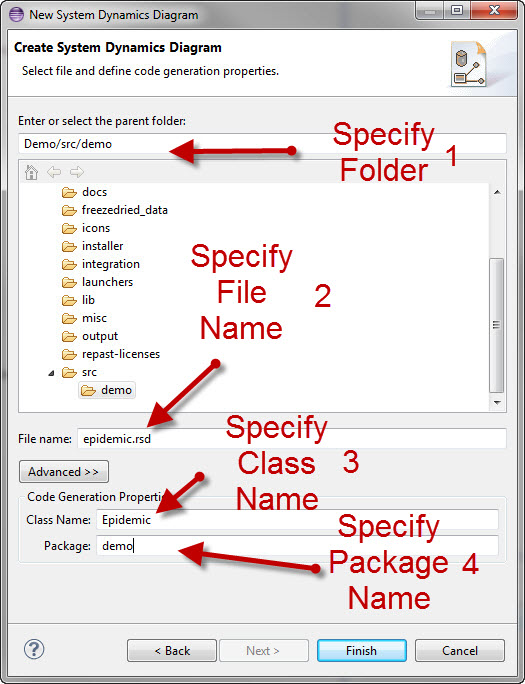
\includegraphics[totalheight=0.35\textheight]{images/008.jpg}
}
\caption{}
\label{fig:008}
\end{center}
\end{figure}

\clearpage

\section{Start Building the Model}
When the wizard completes the process of creating an empty SD model, the diagram tab for the model will appear (See Figure 9). On the right side of the panel, there is a set of SD objects that can be used in the SD model. There are: Influence Arrows, Rates, Stocks, Constants, Variables, Clouds, and Lookups.


\begin{figure}[ht]
\begin{center}
\vspace{.2in}
\centerline {
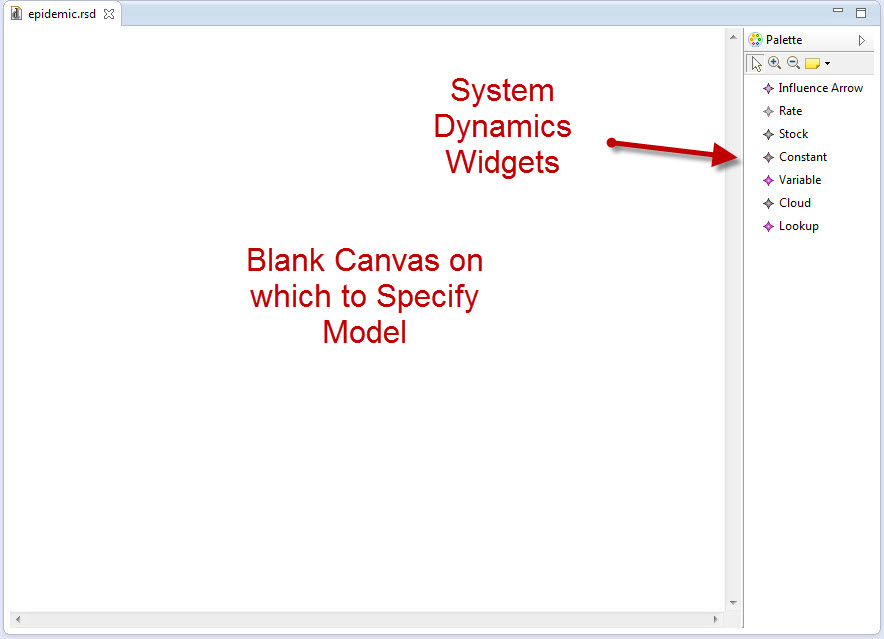
\includegraphics[totalheight=0.5\textheight]{images/009.jpg}
}
\caption{}
\label{fig:009}
\end{center}
\end{figure}

\section{Add a stock}
Begin the process of building the SD model by clicking on the Stock object in the Palette and then click anywhere in the diagram panel to place the stock into it. You will be placed into the mode in which you specify the variable name for the stock. Enter Healthy and hit enter. See Figures 10, 11, and 12.



\begin{figure}[ht]
\begin{center}
\vspace{.2in}
\centerline {
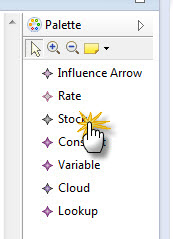
\includegraphics{images/010.jpg}
}
\caption{}
\label{fig:010}
\end{center}
\end{figure}




\begin{figure}[ht]
\begin{center}
\vspace{.2in}
\centerline {

\includegraphics[totalheight=0.15\textheight]{images/011.jpg}
}
\caption{}
\label{fig:011}
\end{center}
\end{figure}




\begin{figure}[ht]
\begin{center}
\vspace{.2in}
\centerline {
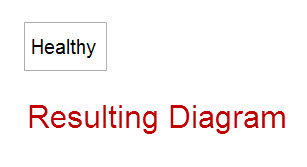
\includegraphics[totalheight=0.15\textheight]{images/012.jpg}
}
\caption{}
\label{fig:012}
\end{center}
\end{figure}

\clearpage

\section{Variable Properties}
Select the Properties tab in the bottom panel of the Eclipse IDE (See Figure 13). The required data for the stock variable are:

\begin{enumerate}
\item Name (set to name you specified).
\item Type (set to stock since variable was declared as stock).
\item Units for the Left Hand Side (LHS) of equation.
\item LHS of equation (Initially set to Name – you might change this depending on the structure of your model – e.g. using arrays)
\item The single argument for the INTEG function. Note that any legal expression that results in one double value is allowable.
\item An Initial Value
\end{enumerate}
\vspace{.2in}

Comments are optional, though recommended.  Functions and Influencing variables are for convenience. Since no influence arrows have been included in the model as of yet, this list box is empty.






\begin{figure}[ht]
\begin{center}
\vspace{.2in}
\centerline {
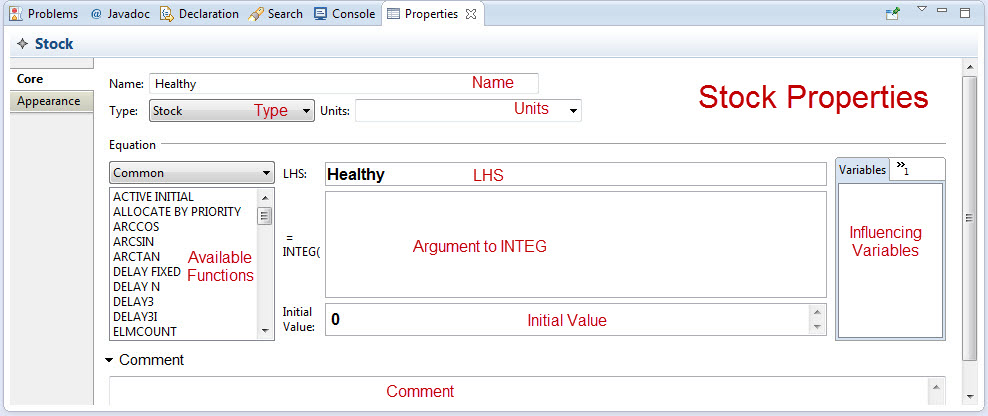
\includegraphics[totalheight=0.4\textheight]{images/013.jpg}
}
\caption{}
\label{fig:013}
\end{center}
\end{figure}

\clearpage

\section{Completing the Diagram}
At this point, create additional model structure Click on object in pallete and then click on diagram to insert it. To create an arrow or rate, click on pallete object, click on the arrow source and hold the mouse button down while moving the cursor to the destination variable and release the mouse button. Rates require a name. Influence arrows do not.

\begin{enumerate}
\item Create a constant named “initial susceptible”
\item Create another stock named “Infected”
\item Create an influence arrow from “initial susceptible” to “Health”
\item Create a rate arrow between “Healthy” and “Infected”
\end{enumerate}
\vspace{.2in}

You should see something like Figure 14.



\begin{figure}[ht]
\begin{center}
\vspace{.2in}
\centerline {
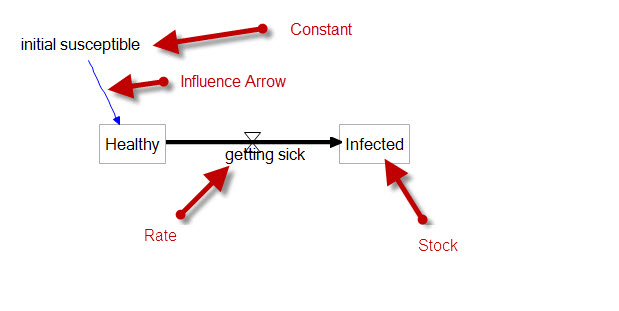
\includegraphics[totalheight=0.15\textheight]{images/014.jpg}
}
\caption{}
\label{fig:014}
\end{center}
\end{figure}




\begin{figure}[ht]
\begin{center}
\vspace{.2in}
\centerline {
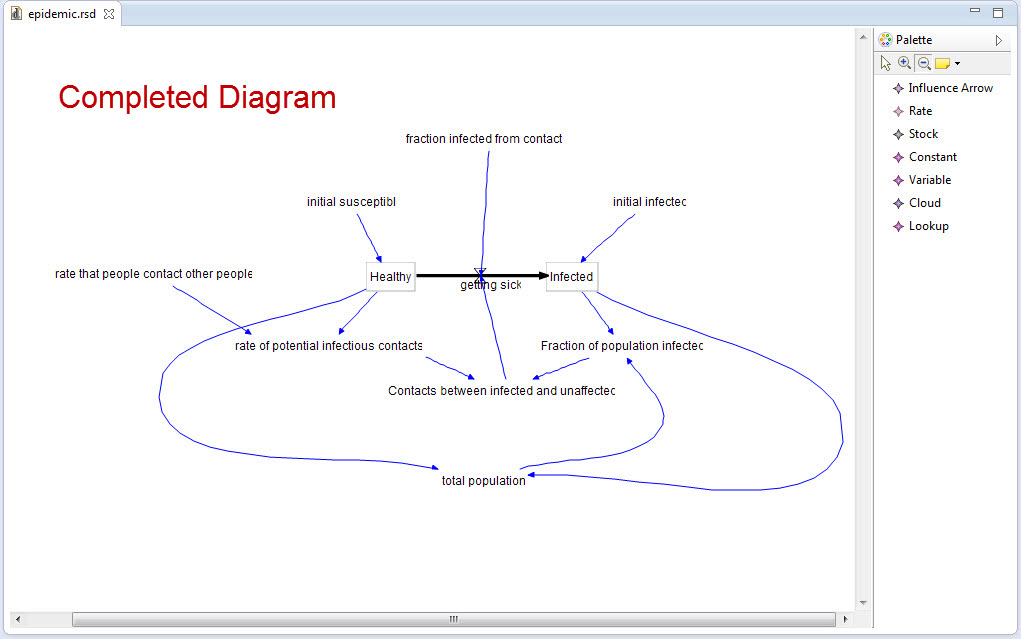
\includegraphics[totalheight=0.3\textheight]{images/015.jpg}
}
\caption{}
\label{fig:015}
\end{center}
\end{figure}

\clearpage

\section{System Level Model Parameters}
Each SD model has a set of required parameters. They are the model start and end times, the integration interval, the reporting interval and finally the unit of time. These are specified on the System Model properties tab. This tab becomes available by clicking in any empty area of the SD model diagram. See Figure 16.





\begin{figure}[ht]
\begin{center}
\vspace{.2in}
\centerline {
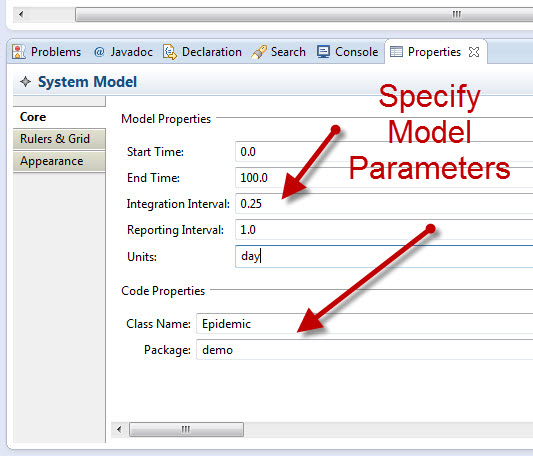
\includegraphics[totalheight=0.4\textheight]{images/016.jpg}
}
\caption{}
\label{fig:016}
\end{center}
\end{figure}

\clearpage


\section{Specifying Variable Properties}
Now that the model structure is complete, it is time to specify the data for all the variables. Start with the Healthy stock (Figure 17).



\begin{figure}[ht]
\begin{center}
\vspace{.2in}
\centerline {
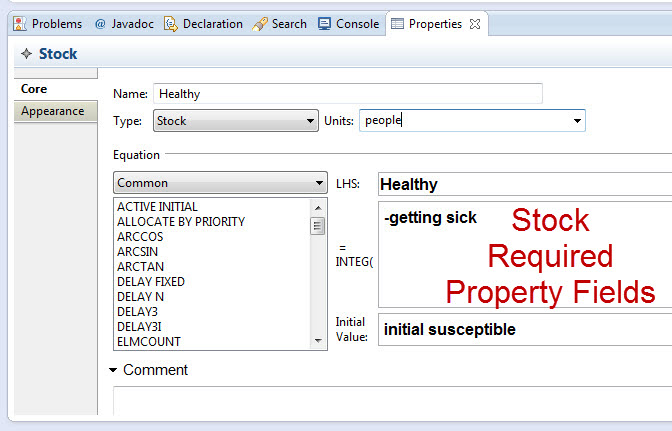
\includegraphics[totalheight=0.3\textheight]{images/017.jpg}
}
\caption{}
\label{fig:017}
\end{center}
\end{figure}

Then getting sick (Figure 18).


\begin{figure}[ht]
\begin{center}
\vspace{.2in}
\centerline {
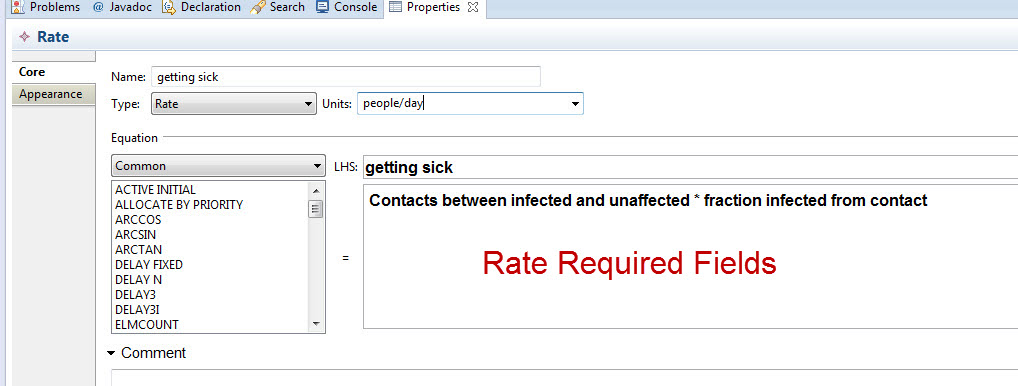
\includegraphics[totalheight=0.3\textheight]{images/018.jpg}
}
\caption{}
\label{fig:018}
\end{center}
\end{figure}

\clearpage

Then fraction infected from contact (Figure 19).


\begin{figure}[ht]
\begin{center}
\vspace{.2in}
\centerline {
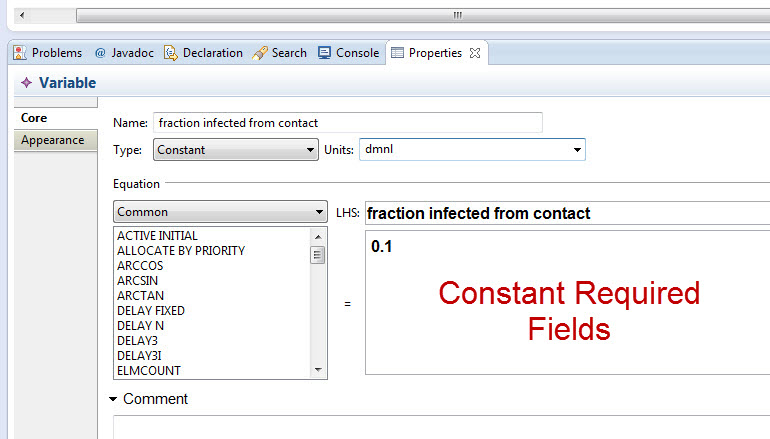
\includegraphics[totalheight=0.3\textheight]{images/019.jpg}
}
\caption{}
\label{fig:019}
\end{center}
\end{figure}

Then contacts between infected and unaffected (Figure 20). To illustrate the consistency check, leave the units field blank for now.


\begin{figure}[ht]
\begin{center}
\vspace{.2in}
\centerline {
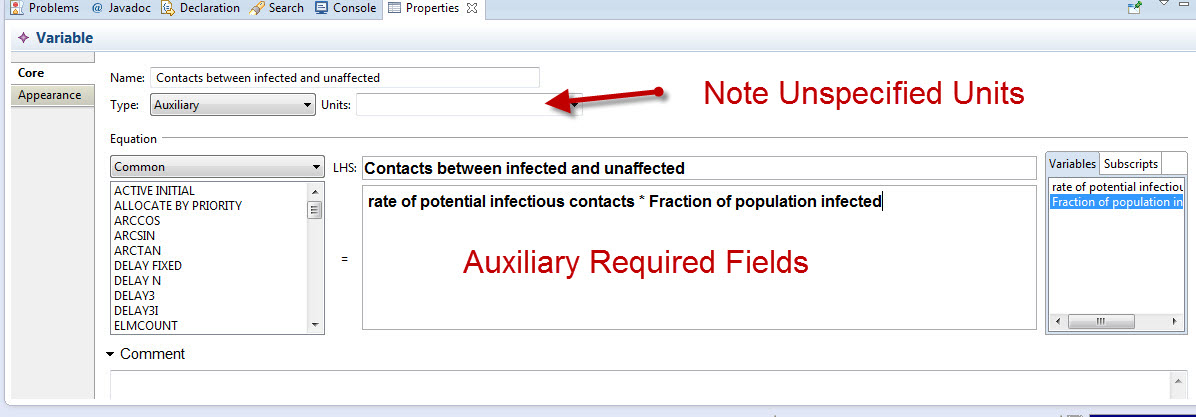
\includegraphics[totalheight=0.3\textheight]{images/020.jpg}
}
\caption{}
\label{fig:020}
\end{center}
\end{figure}

\section{All Model Equations}
Complete the properties for all the variables in the model. Here is a complete specification of the equations and units.

\begin{verbatim}
rate that people contact other people= 5
	1/day
	
Contacts between infected and unaffected = 
rate of potential infectious contacts  * Fraction of population infected
people/day

Infected  = INTEG (getting sick, initial infected)
	people

total population = Healthy + Infected
	people

fraction infected from contact = 0.1
	dmnl

Fraction of population infected = Infected / total population
	dmnl

getting sick = Contacts between infected and unaffected  * 
                      fraction infected from contact
	people /day

initial infected = 10
	people

initial susceptible = 1e+006
	people	

rate of potential infectious contacts = Healthy  
                   * rate that people contact other people
	people /day

Healthy = INTEG( - getting sick, initial susceptible)
	people
\end{verbatim}
 
\clearpage

\section{Checking Model Consistency}
Check the consistency of the SD model (Figure 21).



\begin{figure}[ht]
\begin{center}
\vspace{.2in}
\centerline {
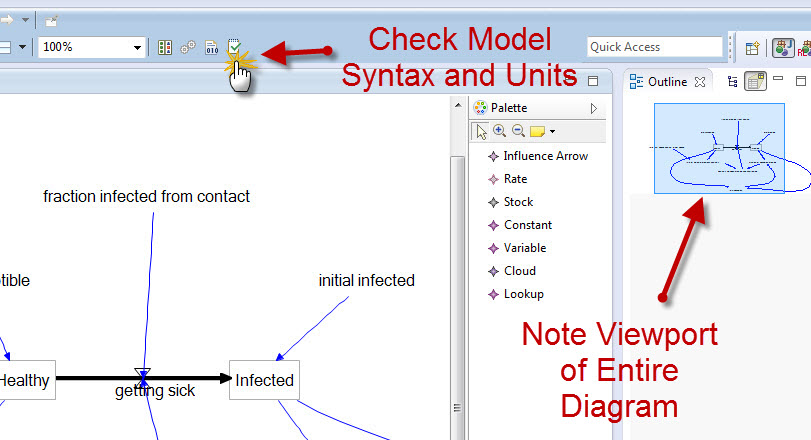
\includegraphics[totalheight=0.4\textheight]{images/021.jpg}
}
\caption{}
\label{fig:021}
\end{center}
\end{figure}


There are inconsistencies in the model. Specifically, Contacts between infected and unaffected does not have its units specified. (Figure 22). Set the Units to people/day (Figure 23).

\clearpage


\begin{figure}[ht]
\begin{center}
\vspace{.2in}
\centerline {
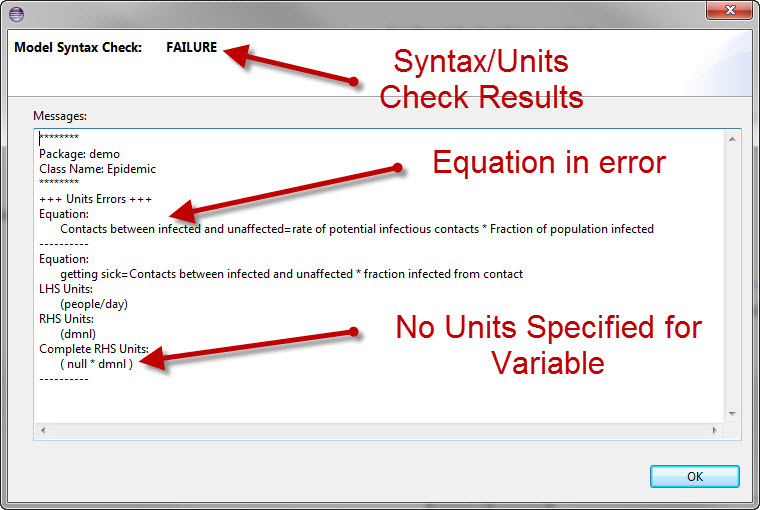
\includegraphics[totalheight=0.3\textheight]{images/022.jpg}
}
\caption{}
\label{fig:022}
\end{center}
\end{figure}




\begin{figure}[ht]
\begin{center}
\vspace{.2in}
\centerline {
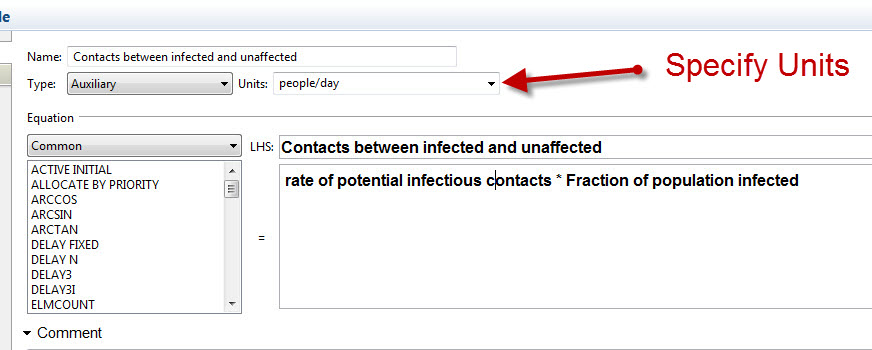
\includegraphics[totalheight=0.3\textheight]{images/023.jpg}
}
\caption{}
\label{fig:023}
\end{center}
\end{figure}

Check for model consistency once again. The model is found to be consistent. (Figure 24).


\begin{figure}[ht]
\begin{center}
\vspace{.2in}
\centerline {
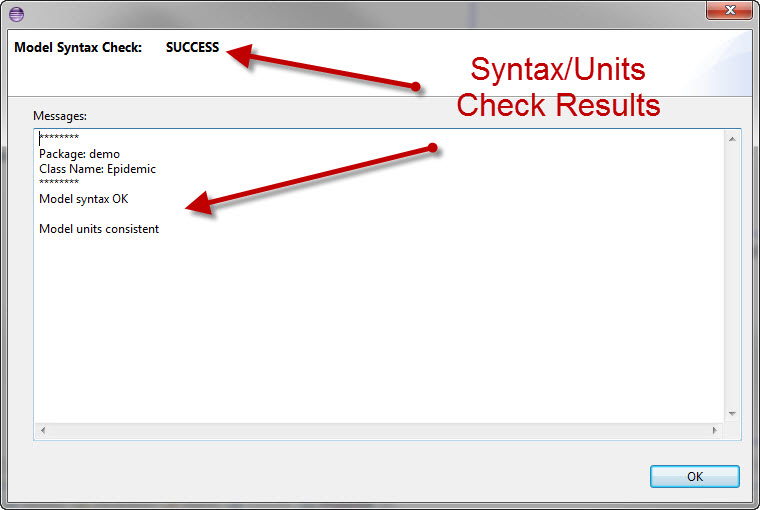
\includegraphics[totalheight=0.3\textheight]{images/024.jpg}
}
\caption{}
\label{fig:024}
\end{center}
\end{figure}

\section{Generate the Java Code}
Now generate the code (See Figure 21, icon to the left of check consistency). Files other than source code will be generated in the scenario directory by Repast Simphony. Among these are:

\begin{enumerate}
\item context.xml
\item parameters.xml
\item repast.simphony.action.data\_set\_0.xml
\item repast.simphony.dataLoader.engine.ClassNameDataLoaderAction\_1.xml
\item scenario.xml
\item usath.xm
\end{enumerate}
\vspace{.2in}

Other files can be created in this directory when you create objects such as graphs and output files through the Repast Simphony GUI when you run the model. The user is prompted whether ir not the scenario directory will be reinitialized to its default contents. (Figure 25).


\begin{figure}[ht]
\begin{center}
\vspace{.2in}
\centerline {
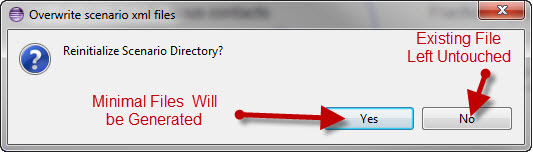
\includegraphics[totalheight=0.1\textheight]{images/025.jpg}
}
\caption{}
\label{fig:025}
\end{center}
\end{figure}

The Java source code and scenario files have been successfully been generated (Figure 26). Figure 27 shows the generated Java source code and scenario files.

\begin{figure}[ht]
\begin{center}
\vspace{.2in}
\centerline {
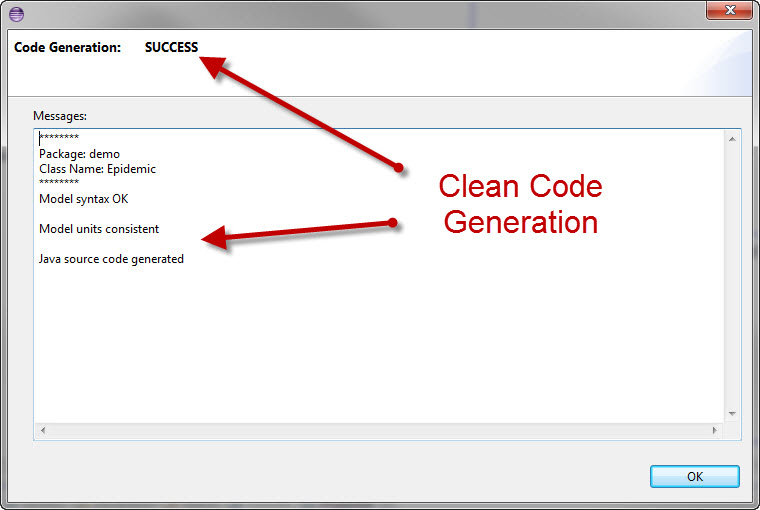
\includegraphics[totalheight=0.3\textheight]{images/026.jpg}
}
\caption{}
\label{fig:026}
\end{center}
\end{figure}




\begin{figure}[ht]
\begin{center}
\vspace{.2in}
\centerline {
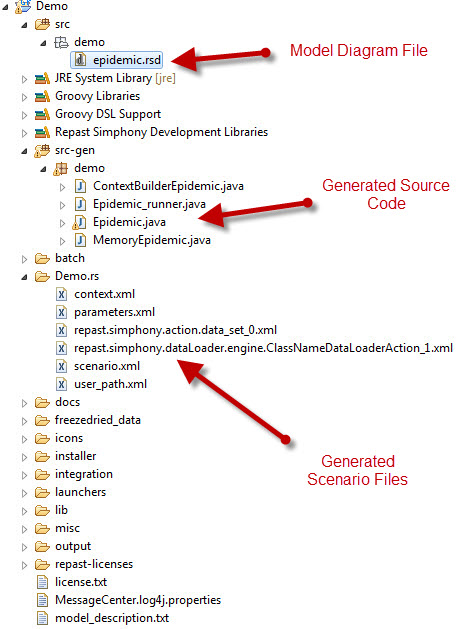
\includegraphics[totalheight=0.45\textheight]{images/027.jpg}
}
\caption{}
\label{fig:027}
\end{center}
\end{figure}


Figure 28 contains the declaration of the model variables and sample getters. Note that the variable names you specified in the equations have been altered to be legal Java variable names.


\begin{figure}[ht]
\begin{center}
\vspace{.2in}
\centerline {
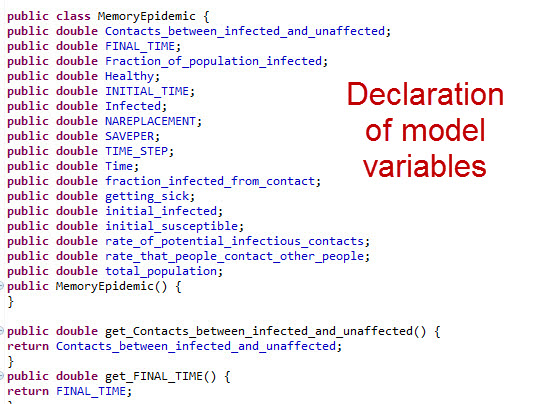
\includegraphics[totalheight=0.3\textheight]{images/028.jpg}
}
\caption{}
\label{fig:028}
\end{center}
\end{figure}


Any variable that has a numeric constant as its value will be placed into the parameters.xml file so that these values can be set via the RS GUI rather than having to edit the diagram and regenerate the code. Figure 29 contains a code sample for extracting this data from the parameters.xml file.

\begin{figure}[ht]
\begin{center}
\vspace{.2in}
\centerline {
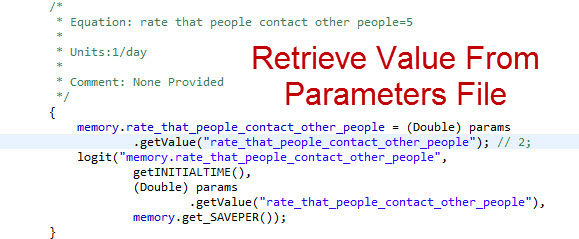
\includegraphics[totalheight=0.3\textheight]{images/029.jpg}
}
\caption{}
\label{fig:029}
\end{center}
\end{figure}


Figure 30 shows a code sample for the implementation of a stock variable.

\begin{figure}[ht]
\begin{center}
\vspace{.2in}
\centerline {
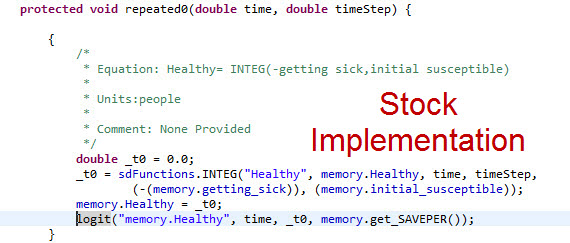
\includegraphics[totalheight=0.3\textheight]{images/030.jpg}
}
\caption{}
\label{fig:030}
\end{center}
\end{figure}

Figure 31 contains the source code for the ContextBuilder.

\begin{figure}[ht]
\begin{center}
\vspace{.2in}
\centerline {
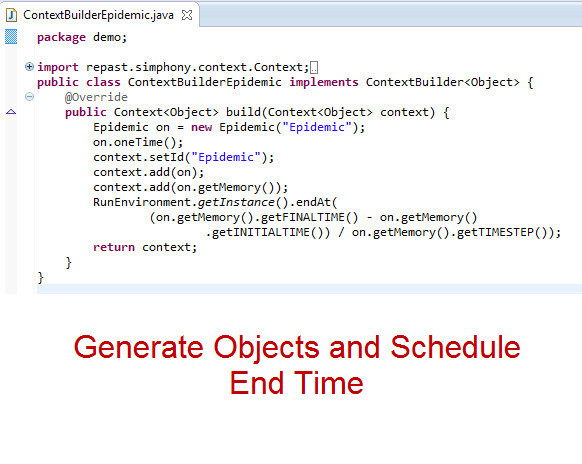
\includegraphics[totalheight=0.3\textheight]{images/031.jpg}
}
\caption{}
\label{fig:031}
\end{center}
\end{figure}

Figure 32 shows the parameters.xnl file that was generated. Note that the values specified in the SD model diagram have been incorporated in to the parameters file.


\begin{figure}[ht]
\begin{center}
\vspace{.2in}
\centerline {
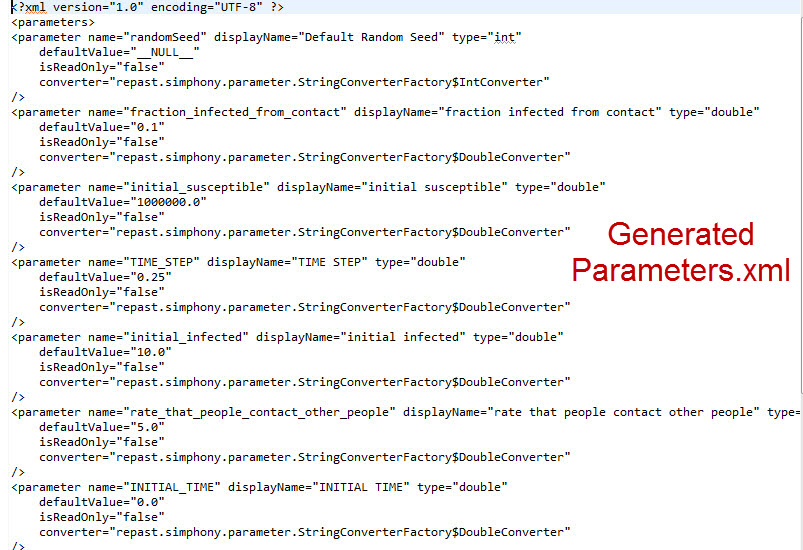
\includegraphics[totalheight=0.4\textheight]{images/032.jpg}
}
\caption{}
\label{fig:032}
\end{center}
\end{figure}

Figure 33 contains a portion of the automatically generated data set for the variables that are used in the model. This is for the convenience of the user in creating reports and graphs. 

\clearpage

\begin{figure}[ht]
\begin{center}
\vspace{.2in}
\centerline {
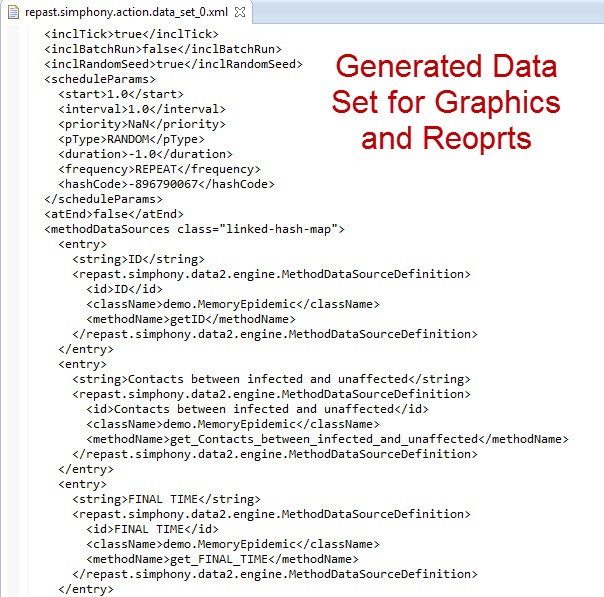
\includegraphics[totalheight=0.5\textheight]{images/033.jpg}
}
\caption{}
\label{fig:033}
\end{center}
\end{figure}

\newpage

\section{Execute the Model}
At this point, the model is ready to be executed. Figure 34 shows the procedure for executing the model using the automatically generated launcher (available through the run>configurations menu item or via the run configurations shortcut).


\begin{figure}[ht]
\begin{center}
\vspace{.2in}
\centerline {
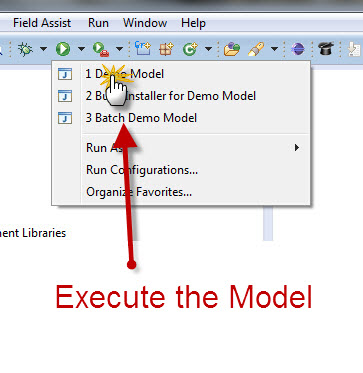
\includegraphics[totalheight=0.3\textheight]{images/034.jpg}
}
\caption{}
\label{fig:034}
\end{center}
\end{figure}


Figure 35 shows the Repast Simphony GUI at startup time. In the scenario tree panel, you can see the generated ContextBuilder and the predefined data set. 

\begin{figure}[ht]
\begin{center}
\vspace{.2in}
\centerline {
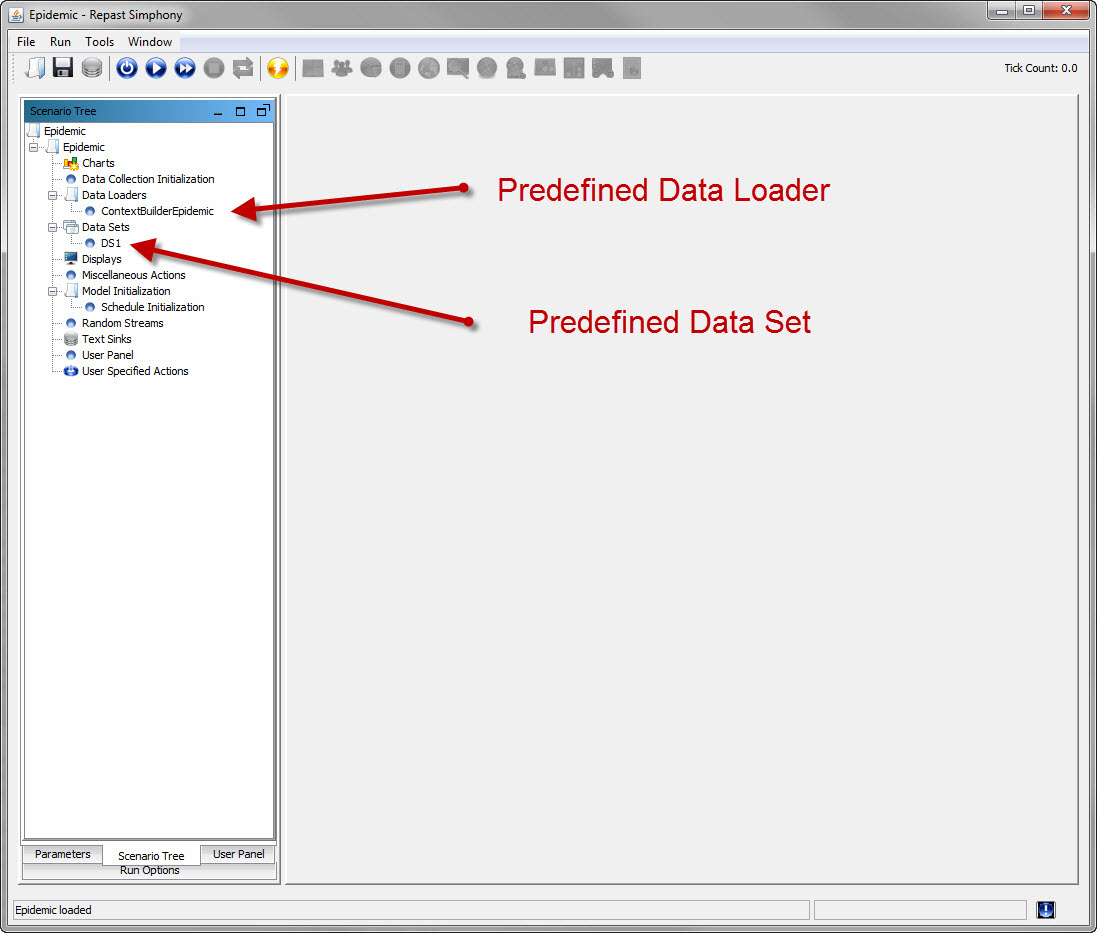
\includegraphics[totalheight=0.3\textheight]{images/035.jpg}
}
\caption{}
\label{fig:035}
\end{center}
\end{figure}

Let’s first create a time series graph so that we can view the results of the model. Figures 36-39 illustrate the process of defining the graph.


\begin{figure}[ht]
\begin{center}
\vspace{.2in}
\centerline {
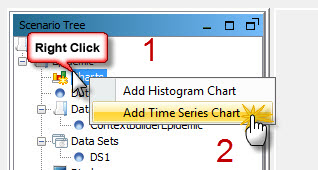
\includegraphics[totalheight=0.3\textheight]{images/036.jpg}
}
\caption{}
\label{fig:036}
\end{center}
\end{figure}

Specify any name that you would like and use the predefined data set.


\begin{figure}[ht]
\begin{center}
\vspace{.2in}
\centerline {
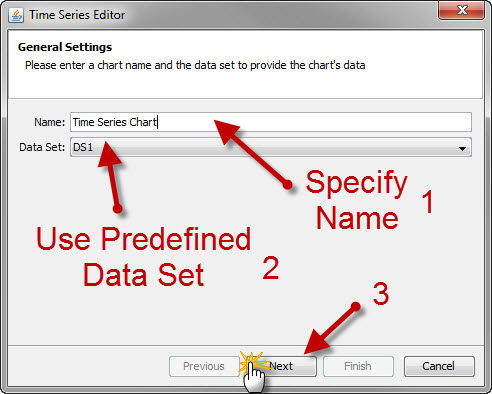
\includegraphics[totalheight=0.3\textheight]{images/037.jpg}
}
\caption{}
\label{fig:037}
\end{center}
\end{figure}


Select Healthy, Infected, and getting sick from the left hand side of the shuttle and transfer them to the right hand side. Click Next to continue.


\begin{figure}[ht]
\begin{center}
\vspace{.2in}
\centerline {
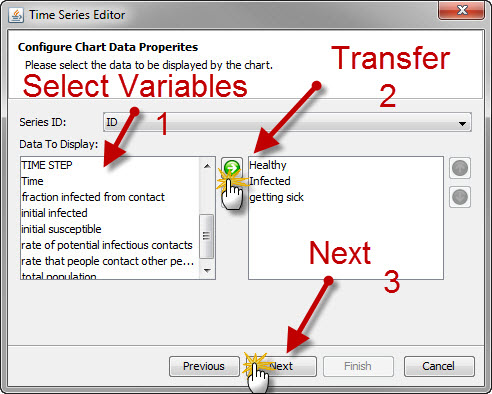
\includegraphics[totalheight=0.3\textheight]{images/038.jpg}
}
\caption{}
\label{fig:038}
\end{center}
\end{figure}


Specify the Title and Y Axis label. Click finish to complete the graph definition. Remember to save the scenario. If you do not save the scenario, this information will be lost if you either exit Repast Simphony or reinitialize the model.

\begin{figure}[ht]
\begin{center}
\vspace{.2in}
\centerline {
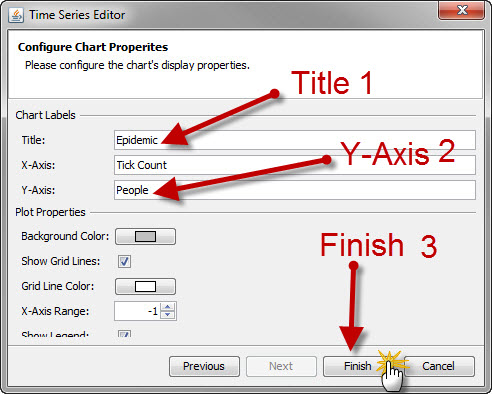
\includegraphics[totalheight=0.3\textheight]{images/039.jpg}
}
\caption{}
\label{fig:039}
\end{center}
\end{figure}

Figure 40 shows the process for initializing the model. This consists of access the scenario files and initializing all the variables that can be initialized at this time. In addition, the graph we defined will be displayed (Figure 41). Note that you can start the model without initializing it. The initialization process will take place, but this can happen so quickly that the GUI will not be able to display a graph before the model reaches its end time. It is recommended that you always initialize the model before starting it.


\begin{figure}[ht]
\begin{center}
\vspace{.2in}
\centerline {
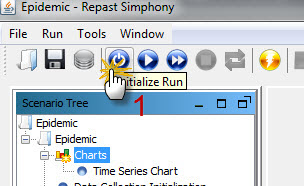
\includegraphics[totalheight=0.3\textheight]{images/040.jpg}
}
\caption{}
\label{fig:040}
\end{center}
\end{figure}

Figure 41 shows the GUI after the model has been initialized.


\begin{figure}[ht]
\begin{center}
\vspace{.2in}
\centerline {
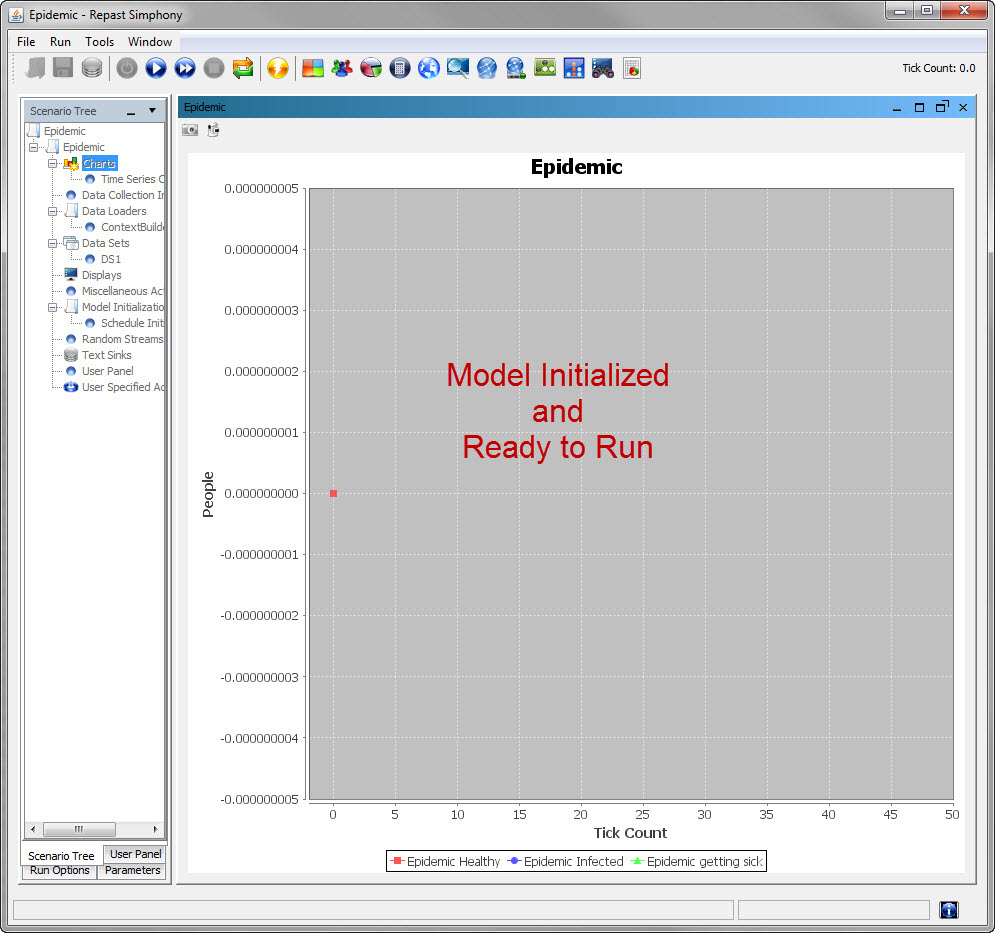
\includegraphics[totalheight=0.3\textheight]{images/041.jpg}
}
\caption{}
\label{fig:041}
\end{center}
\end{figure}

Figure 42 shows the icon to click to start the model execution.


\begin{figure}[ht]
\begin{center}
\vspace{.2in}
\centerline {
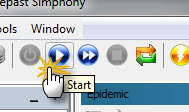
\includegraphics[totalheight=0.3\textheight]{images/042.jpg}
}
\caption{}
\label{fig:042}
\end{center}
\end{figure}

Figure 43 shows the graph being displayed at the end of the model time frame. Note that the graph is updated as the model executes rather than just displaying at the end.


\begin{figure}[ht]
\begin{center}
\vspace{.2in}
\centerline {
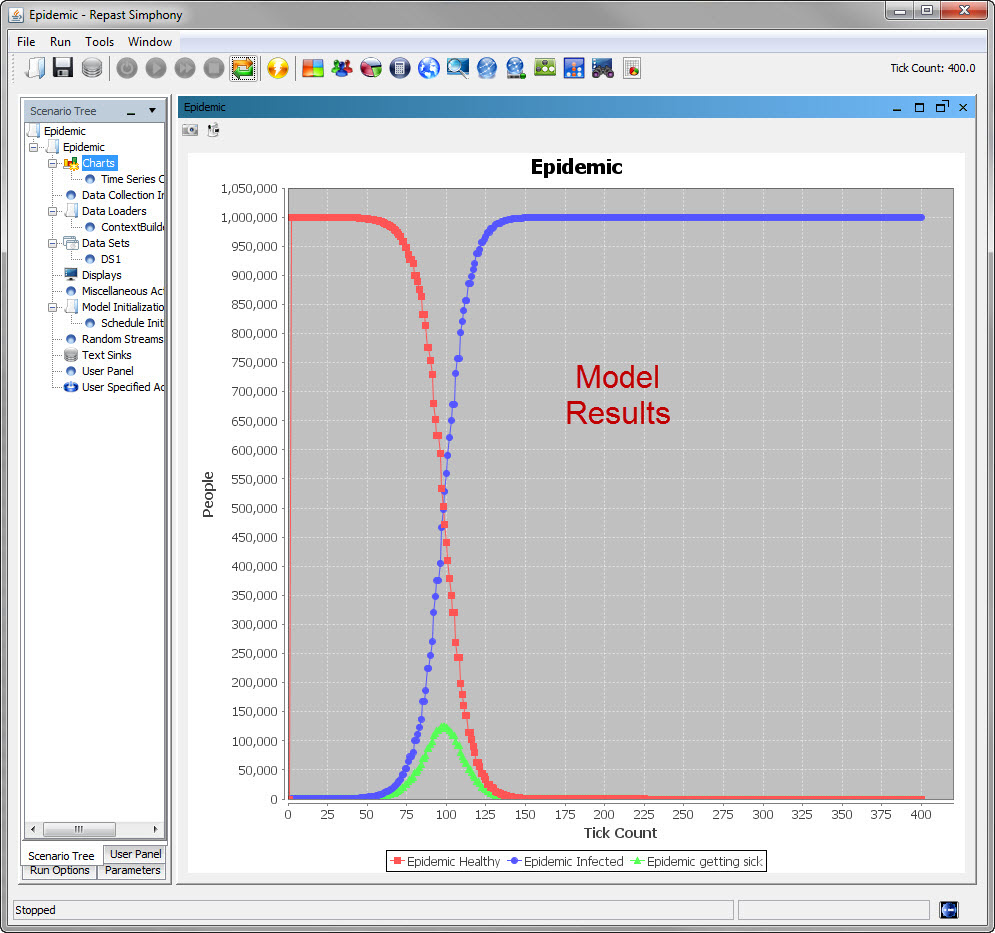
\includegraphics[totalheight=0.5\textheight]{images/043.jpg}
}
\caption{}
\label{fig:043}
\end{center}
\end{figure}

Figure 44 shows the icon that can be used to reset the model for another execution without having to restart the Repast Simphony GUI.


\begin{figure}[ht]
\begin{center}
\vspace{.2in}
\centerline {
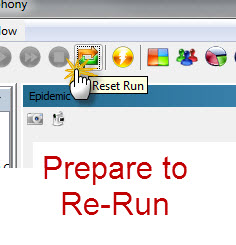
\includegraphics[totalheight=0.2\textheight]{images/044.jpg}
}
\caption{}
\label{fig:044}
\end{center}
\end{figure}

\newpage

\section{Import an Existing System Dynamics Model}
The Repast Simphony System Dynamics subsystem can read the equations and associated data from  mdl files generated by Vensim. This allows Repast Simphony to import existing System Dynamics models into your project. Figure 45 and 46 show the process of importing an existing system dynamics model into Repast Simphony. Note that a file browser pops up to allow the user to select the appropriate file.



\begin{figure}[ht]
\begin{center}
\vspace{.2in}
\centerline {
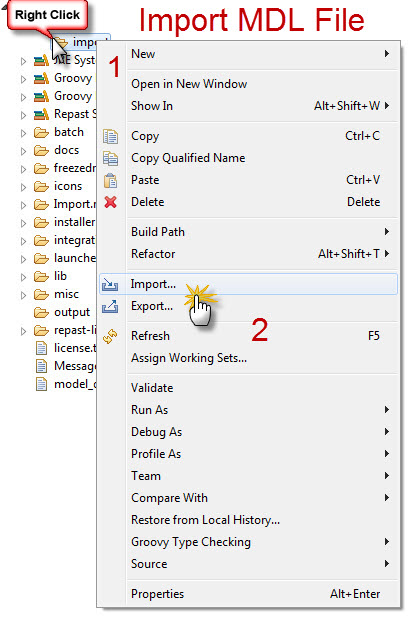
\includegraphics[totalheight=0.6\textheight]{images/045.jpg}
}
\caption{}
\label{fig:045}
\end{center}
\end{figure}


\clearpage

\begin{figure}[ht]
\begin{center}
\vspace{.2in}
\centerline {
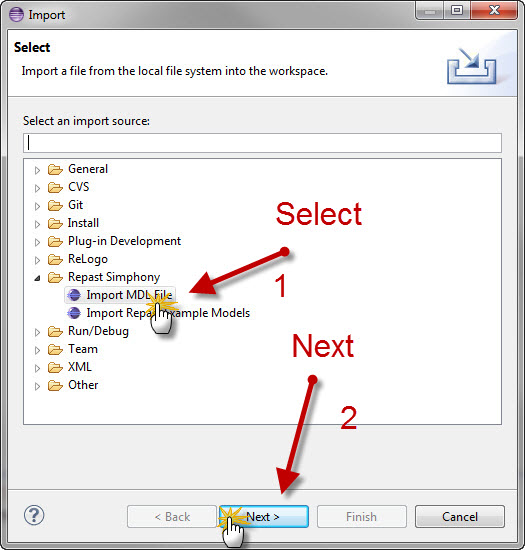
\includegraphics[totalheight=0.3\textheight]{images/046.jpg}
}
\caption{}
\label{fig:046}
\end{center}
\end{figure}

Once imported, the model diagram is displayed as in Figure 47. Note that positional data in the existing SD model is not transferred to Repast Simphony. Rather, the Eclipse diagramming software computes the initial positioning. Components can be rearranged by dragging them to the desired locations. Occasionally, influence arrows will not properly display (i.e. are not visible in the diagram). Minor shifting of the variable’s position normally causes the arrow to be displayed properly on the redraw.


\begin{figure}[ht]
\begin{center}
\vspace{.2in}
\centerline {
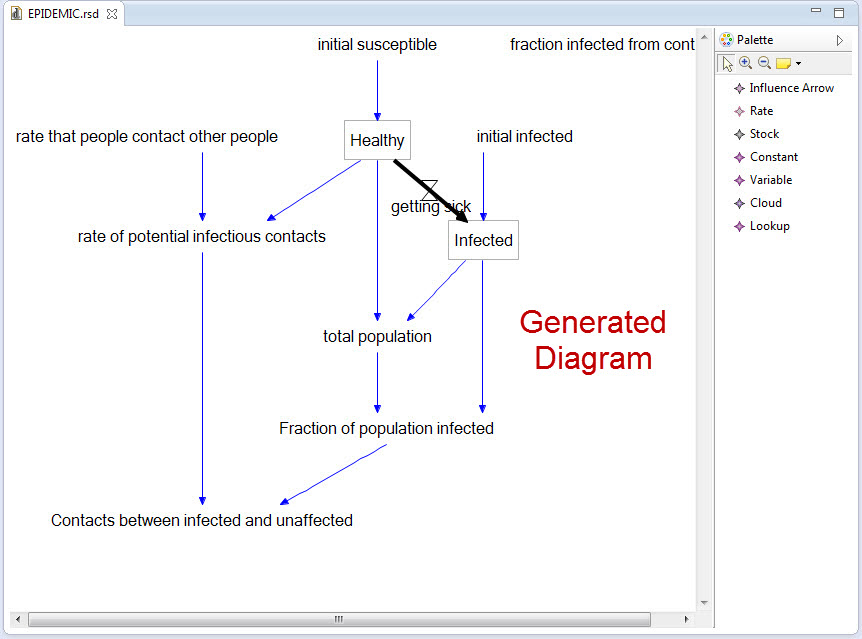
\includegraphics[totalheight=0.3\textheight]{images/047.jpg}
}
\caption{}
\label{fig:047}
\end{center}
\end{figure}




\begin{figure}[ht]
\begin{center}
\vspace{.2in}
\centerline {
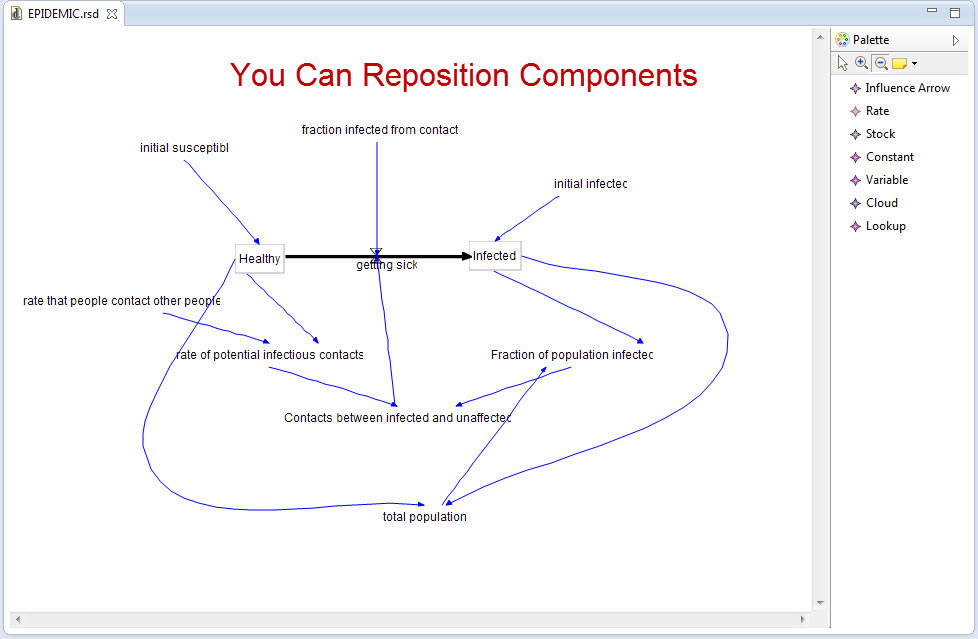
\includegraphics[totalheight=0.3\textheight]{images/048.jpg}
}
\caption{}
\label{fig:048}
\end{center}
\end{figure}

\section{Support for Arrays}
Repast Simphony System Dynamics supports the use of arrays in models. Figures 49-55 show the process for adding arrays to an existing model. First, we need to start the process by creating a subscript (Figure 49).


You must click on the Add button to bring up an empty, unnamed subscript (Figure 50).


Then we can add the name and specify the subscript values as a comma separated list (Figures 51 and 52). Note that subscripts take alphanumeric values. During the code generation phase, these are changed to numeric subscripts. It is intended that this be hidden from the user as the use of mapped subscripts (an advanced SD model technique) can cause the numeric mapping to be less that obvious in some cases.


\begin{figure}[ht]
\begin{center}
\vspace{.2in}
\centerline {
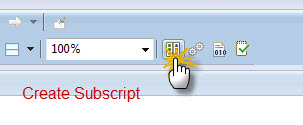
\includegraphics[totalheight=0.3\textheight]{images/052.jpg}
}
\caption{}
\label{fig:052}
\end{center}
\end{figure}

The user needs to specify exactly where each instance of a subscript must appear. Not all variables in an equation that contains arrays need to be subscripted. But once a variable is referenced as an array, it must be referenced as an array in all instances with consistent use of subscripts. Figures 53 and 54 show the process of adding a subscript to an equation. In this case, we want to add the Country subscript to the Healthy stock variable to create an array. Place the cursor in the proper position within the LHS text box and then click on the subscript you wish to insert. The subscript notation is added to the Healthy stock variable.


\begin{figure}[ht]
\begin{center}
\vspace{.2in}
\centerline {
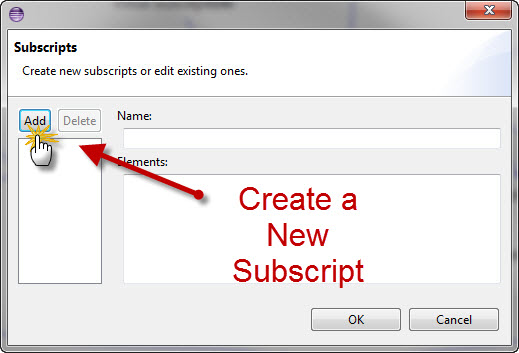
\includegraphics[totalheight=0.3\textheight]{images/053.jpg}
}
\caption{}
\label{fig:053}
\end{center}
\end{figure}


\begin{figure}[ht]
\begin{center}
\vspace{.2in}
\centerline {
\includegraphics[totalheight=0.3\textheight]{images/054.jpg}
}
\caption{}
\label{fig:054}
\end{center}
\end{figure}

As indicated in Figure 55, the subscript notation will be inserting only at the cursor location. If there are multiple variables requiring the subscript notation, each must be added individually.


\begin{figure}[ht]
\begin{center}
\vspace{.2in}
\centerline {
\includegraphics[totalheight=0.3\textheight]{images/055.jpg}
}
\caption{}
\label{fig:055}
\end{center}
\end{figure}


Figure 56 shows on of the possible errors resulting from inconsistent array and non-array references to a variable. The instance of the Healthy stock variable in the rate of potential infectious contacts equation is that of a scalar reference. The consistency checker attempted to find the variable named Healthy in the scalar variable table. But since it had been defined as an array in its LHS definition, the lookup failed and the error is reported. This also occurs for the Infected and total population variables in this example.

\begin{figure}[ht]
\begin{center}
\vspace{.2in}
\centerline {
\includegraphics[totalheight=0.15\textheight]{images/056.jpg}
}
\caption{}
\label{fig:056}
\end{center}
\end{figure}

Note that the existence of arrays in an SD model is not detectable from simply looking at the model diagram as shown in Figure 57. You would need to examine the properties for the variables to determine which are subscripted.

\begin{figure}[ht]
\begin{center}
\vspace{.2in}
\centerline {
\includegraphics[totalheight=0.15\textheight]{images/057.jpg}
}
\caption{}
\label{fig:057}
\end{center}
\end{figure}




\begin{figure}[ht]
\begin{center}
\vspace{.2in}
\centerline {
\includegraphics[totalheight=0.15\textheight]{images/058.jpg}
}
\caption{}
\label{fig:058}
\end{center}
\end{figure}




\begin{figure}[ht]
\begin{center}
\vspace{.2in}
\centerline {
\includegraphics[totalheight=0.35\textheight]{images/059.jpg}
}
\caption{}
\label{fig:059}
\end{center}
\end{figure}




\begin{figure}[ht]
\begin{center}
\vspace{.2in}
\centerline {
\includegraphics[totalheight=0.35\textheight]{images/060.jpg}
}
\caption{}
\label{fig:060}
\end{center}
\end{figure}








\end{document}
